\section{Three-dimensional simulations}\label{results3d}
In this section we review 3D simulations carried 
out using ZEUS-MP and PLUTO. The main purpose is to verify 
the above results with different numerical codes, and validate  
the 2D approximation.    

The 3D disc has radial size
$[r_\mathrm{min},r_\mathrm{max}]=[0.4,10]R_0$ and vertical extent  
$n_H=2$ scale-heights at $R=R_0$. The resolution is $N_r\times N_\theta\times
N_\phi=256\times32\times512$, or about $4$ cells per
$H$. Because of the reduced resolution 
compared to 2D, we use a smooth perturbation by setting
$\delta = 10^{-3}$ and $M=1$ in Eq. \ref{randpert}. This corresponds
to a single $m=1$ disturbance in $R\in[R_1,R_2]$.
%, which
%eventually dominates in 2D simulations.  

The 3D discs are initialised in approximate equilibrium only, so we
first evolve the disc without perturbations using  
$(\lmax,\mmax)=(32,0)$ up to $t=10P_0$, during which 
meridional velocities are damped out. We then restart the simulation
with the above perturbation and $(\lmax,\mmax)=(32,32)$, and damp
meridional velocities near the radial boundaries. 

Fig. \ref{3d_ampmax} plots the evolution of the $m=1$ spiral amplitudes measured
in the ZEUS-MP and PLUTO runs. We also ran simulations
with a strictly isothermal equation of state ($q=0$), which display no
growth compared to that with a temperature gradient.  This confirms
the temperature gradient effect is the same in 3D. 
%why no high m
                                %modes as in 2D for iso disc?
                                %resolution? 

In the ZEUS-MP run, we observed high-$m$ disturbances developed near 
the inner boundary initially, which is likely responsible for the
growth seen at $t<50P_0$. This is a numerical artifact and effectively
seeds the simulation with a larger perturbation. Results
from ZEUS-MP are therefore off-set from PLUTO by $\sim50P_0$. However,
once the coherent $m=1$ spiral begins to grow ($t\gtrsim 100P_0$), 
we measure similar growth rates in both codes: 
\begin{align*}
  &\gamma \simeq 0.0073\Omega_k(R_0) \quad\quad \mathrm{PLUTO},\\
  &\gamma \simeq 0.0085\Omega_k(R_0) \quad\quad \varA{ZEUS-MP}.
\end{align*}
Both are somewhat smaller than the 2D simulations. {\bf This is
  possibily} because of the lower resolutions adopted in 3D {\bf
  and/or because the effective Toomre parameter is larger in 3D which,
  from Eq. \ref{theoretical_rate1}, is stabilising.} 

% and/or the small softening length
% employed in 2D. 
%Rc = 8.6R_0

\begin{figure}
  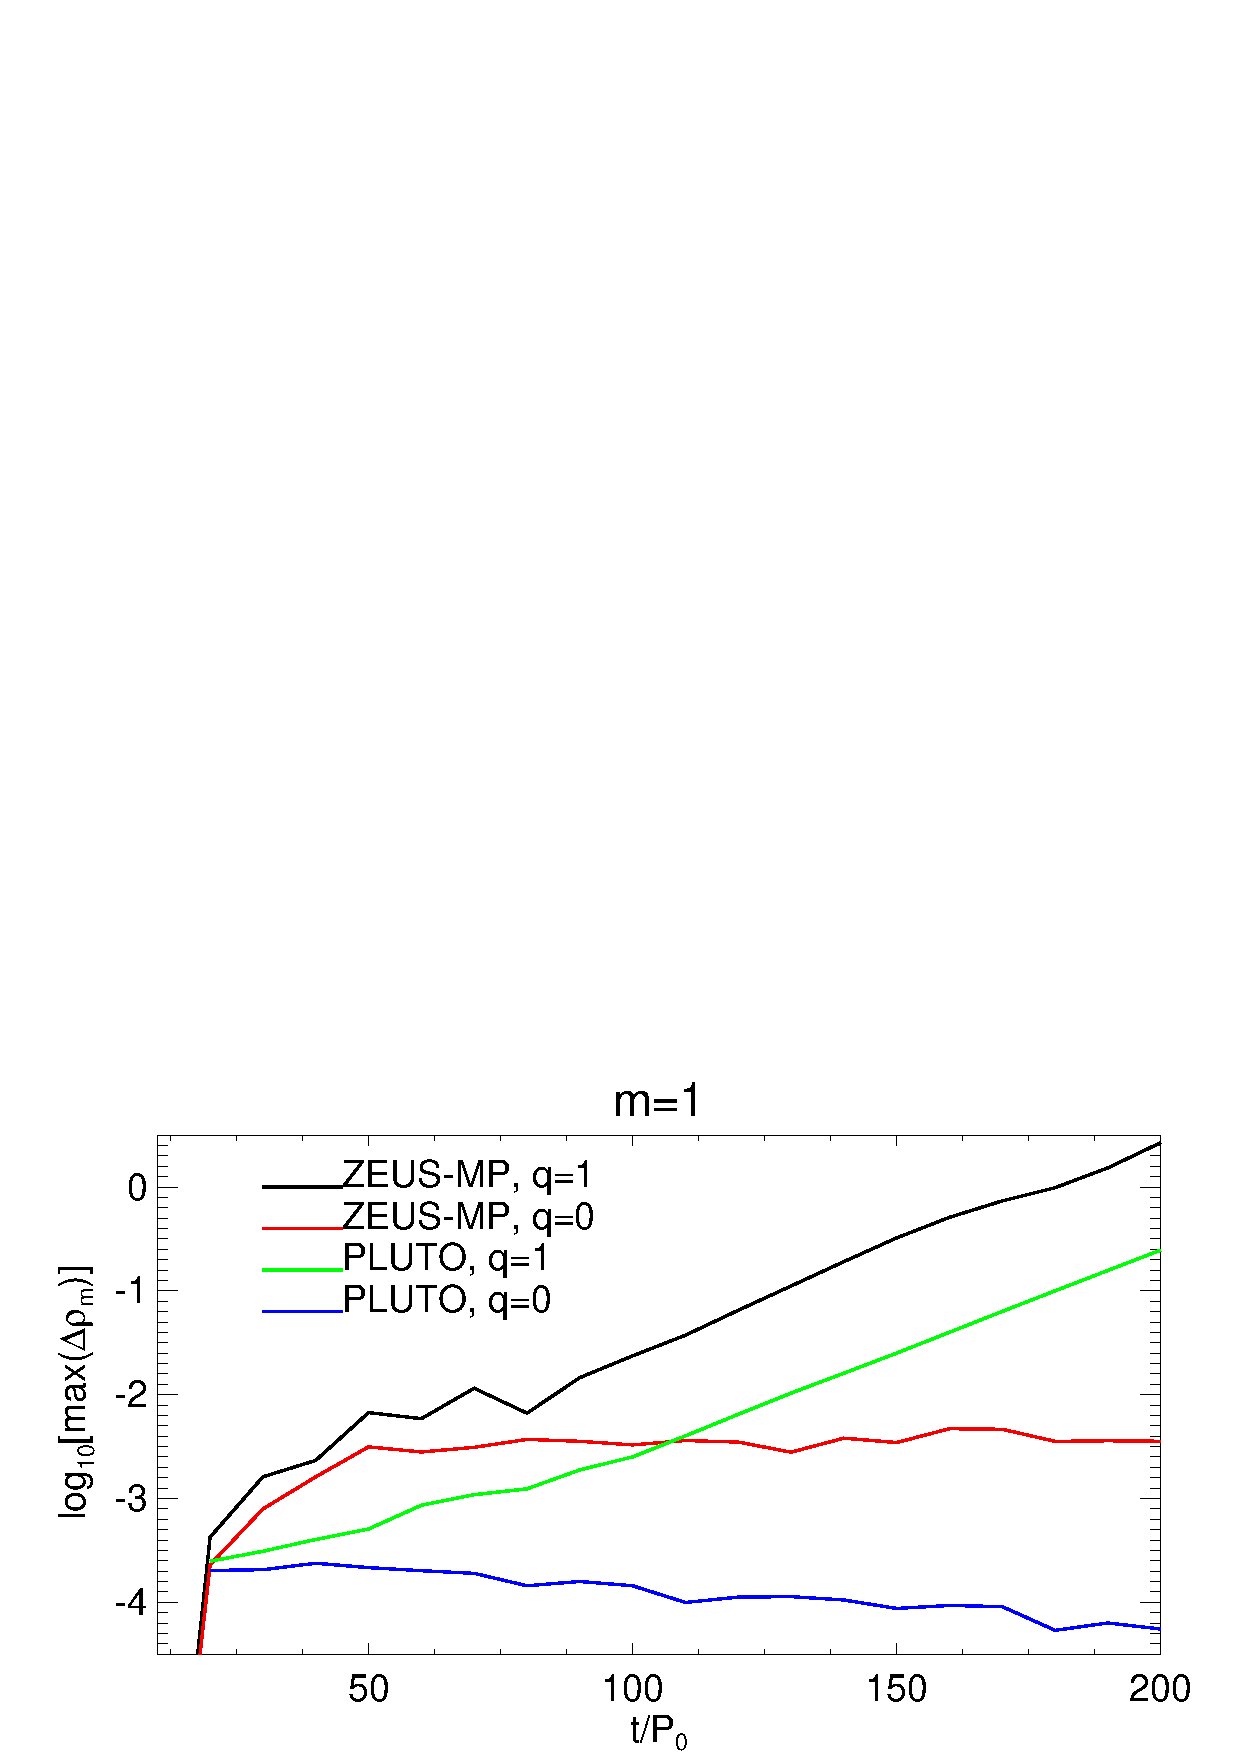
\includegraphics[width=\linewidth]{figures/m1_analysis_plot_ampmax3d}
  \caption{Evolution of the maximum $m=1$ density component in  $r\in[R_1,R_2]$
    in the 3D simulations. Results from discs with a 
    temperature gradient ($q=1$) and a strictly isothermal disc
    ($q=0$) are shown.  
    \label{3d_ampmax}}   
\end{figure}

%more global than 2D?

Visualisations of the 3D simulations are shown in   
Fig. \ref{3d_prelim} for the disc midplane and near the upper disc
boundary. The snapshots are chosen when the one-armed spirals in the two codes
have reached comparable amplitudes. %The agreement between the codes,
%as well as with the 2D simulations (Fig. \ref{2d_fargo_viz}), is
%satisfactory. 
Both codes show similar one-armed patterns at either height, and the
midplane snapshot is similar to the 2D simulation
(Fig. \ref{fargo_2d}). 
The largest spiral amplitude is found in the
self-gravitating region $R\in[R_1,R_2]$, independent of
height. However, notice the spiral pattern extends into 
the non-self-gravitating outer disc ($R>R_2$) at $z\sim 2H$, i.e.    
the disturbance becomes more global away from the midplane.  
%2d only adequate for self-gravitaing region 
\begin{figure}
  \begin{center}
    \subfigure[ZEUS-MP]{
      \includegraphics[scale=0.305,clip=true,trim=0cm 0cm 0cm 0cm]{figures/polarxy2_dens015_z0}  
      \includegraphics[scale=0.305,clip=true,trim=0.8cm 0cm 0cm
      0cm]{figures/polarxy2_dens015_zmax}  
    }
    \subfigure[PLUTO]{
      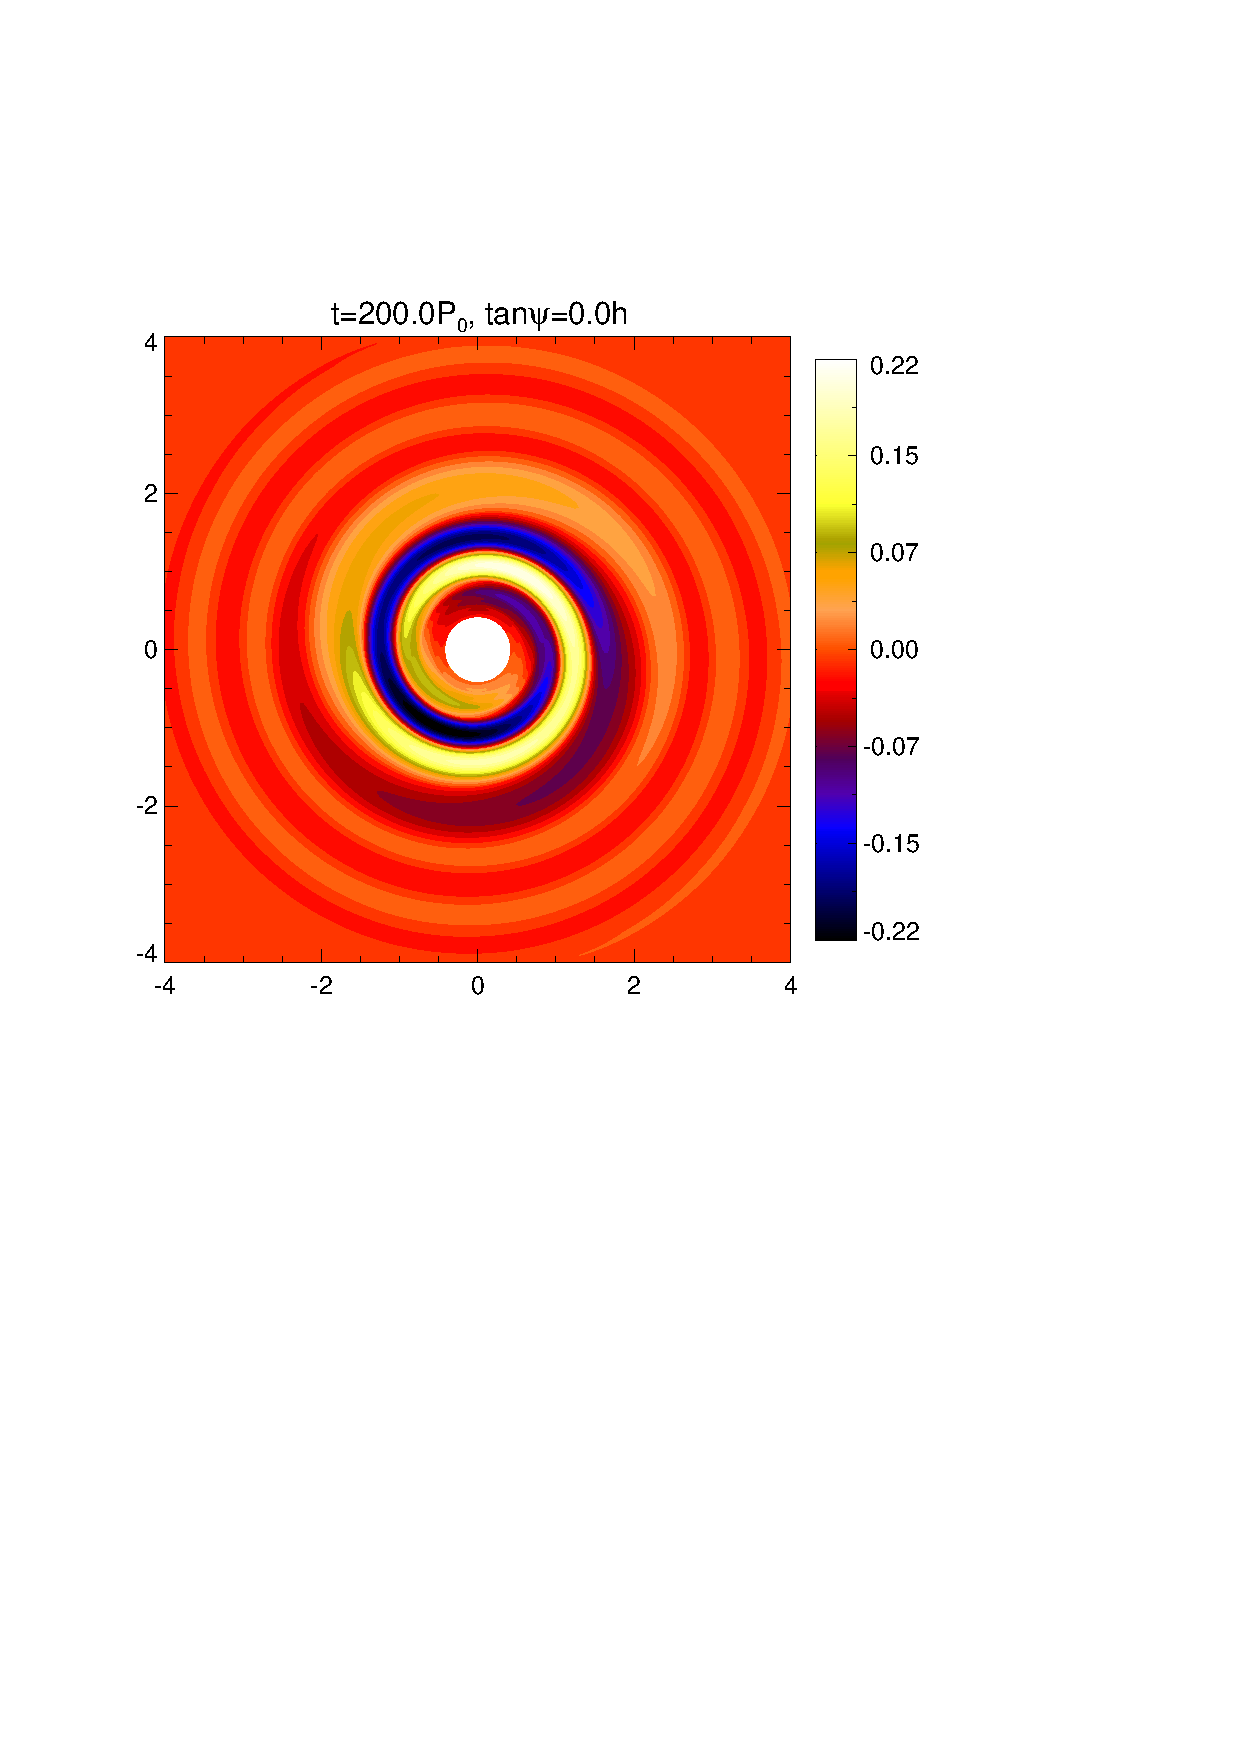
\includegraphics[scale=0.305,clip=true,trim=0cm 0cm 0cm 0cm]{figures/pdiskxy_023_z0}
      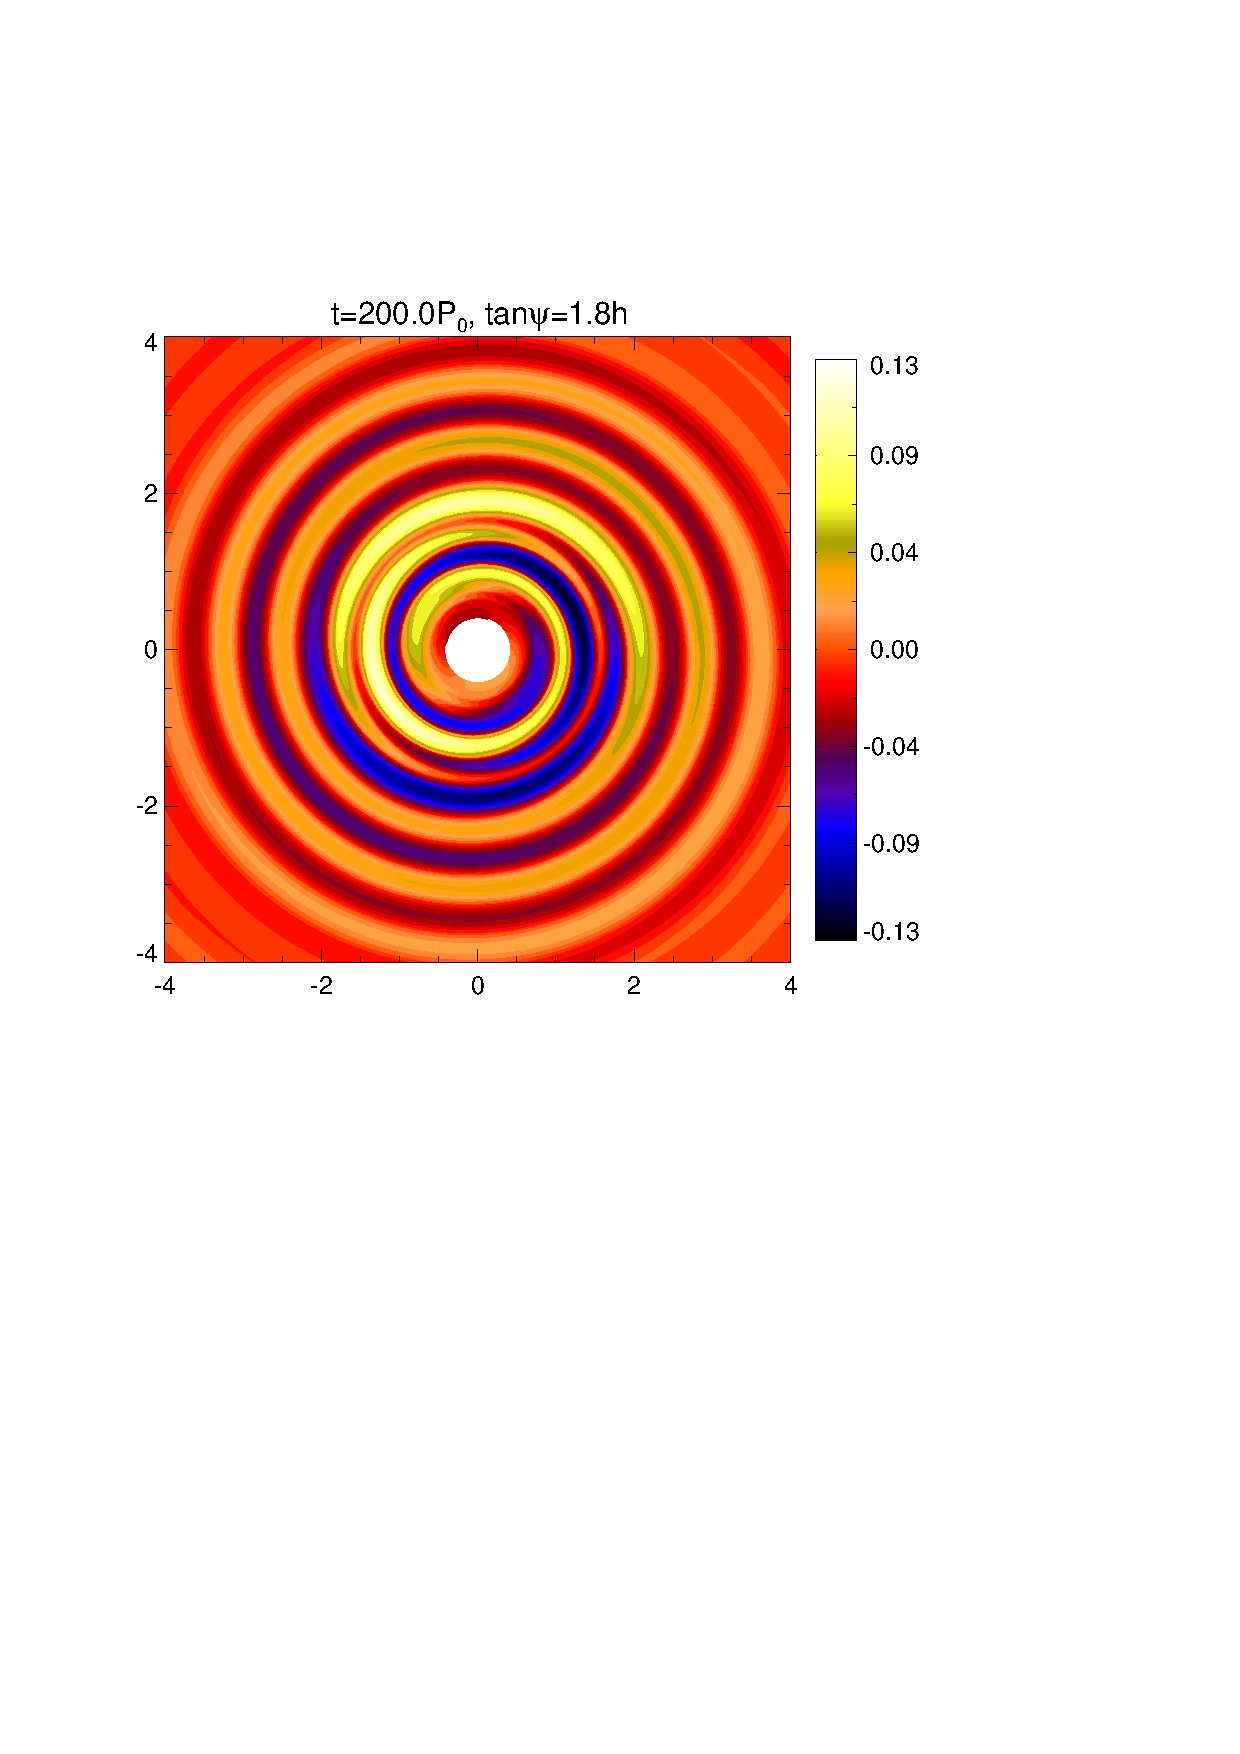
\includegraphics[scale=0.305,clip=true,trim=0.8cm 0cm 0cm
      0cm]{figures/pdiskxy_023_zmax}
    }
  \end{center}
  \caption{Three-dimensional simulations using the ZEUS-MP (top) and 
    PLUTO (bottom) codes. The $m=1$ density component $\Delta\rho_1$
    at the midplane (left) and approximately 
    two scale-heights above the midplane (right) is shown. Here $\psi
    \equiv \pi/2 - \theta$ is the angular height  
    from the midplane. \label{3d_prelim}}   
\end{figure}

\subsection{Vertical structure}
Fig. \ref{3d_rz} shows the vertical structure of the one-armed 
spiral in the PLUTO run. The spiral is vertically confined to $z
\lesssim H$ at $R\sim R_0$ (the self-gravitating region). Thus, a 2D
disc model, representing dynamics near the disc midplane, is  
sufficient capture the instability. However, for $R>2R_0$ the spiral amplitude
increases away from the midplane. It remains  
small in our disc model ($|\Delta\rho_1| \lesssim 0.1$), but could become 
significant with a larger vertical domain. This means that 3D 
simulations are necessary to study the effect of the one-armed spiral
on the exterior, non-self-gravitating disc.  
   
\begin{figure}
  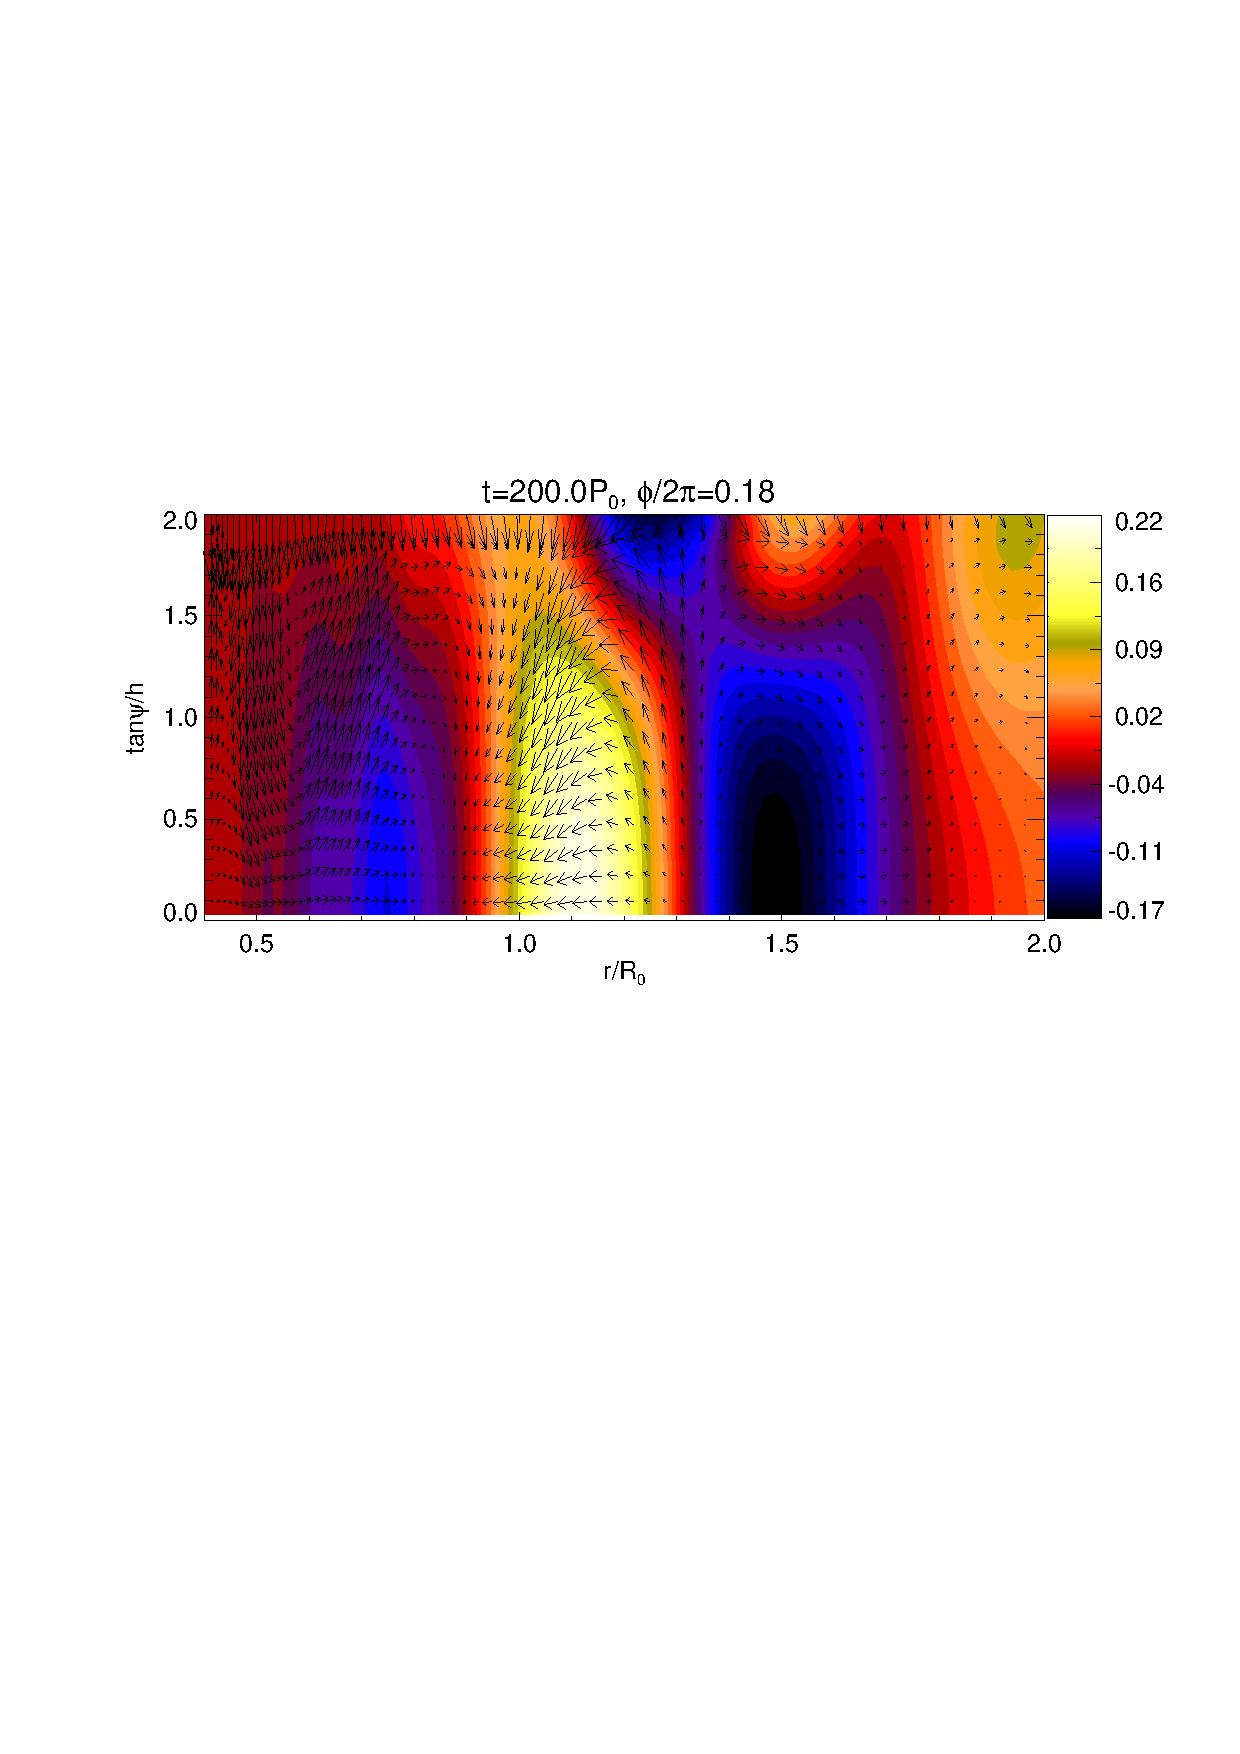
\includegraphics[scale=0.47,clip=true,trim=0cm 0.79cm 0cm
  0cm]{figures/pdisk_rz_023_sg}  
  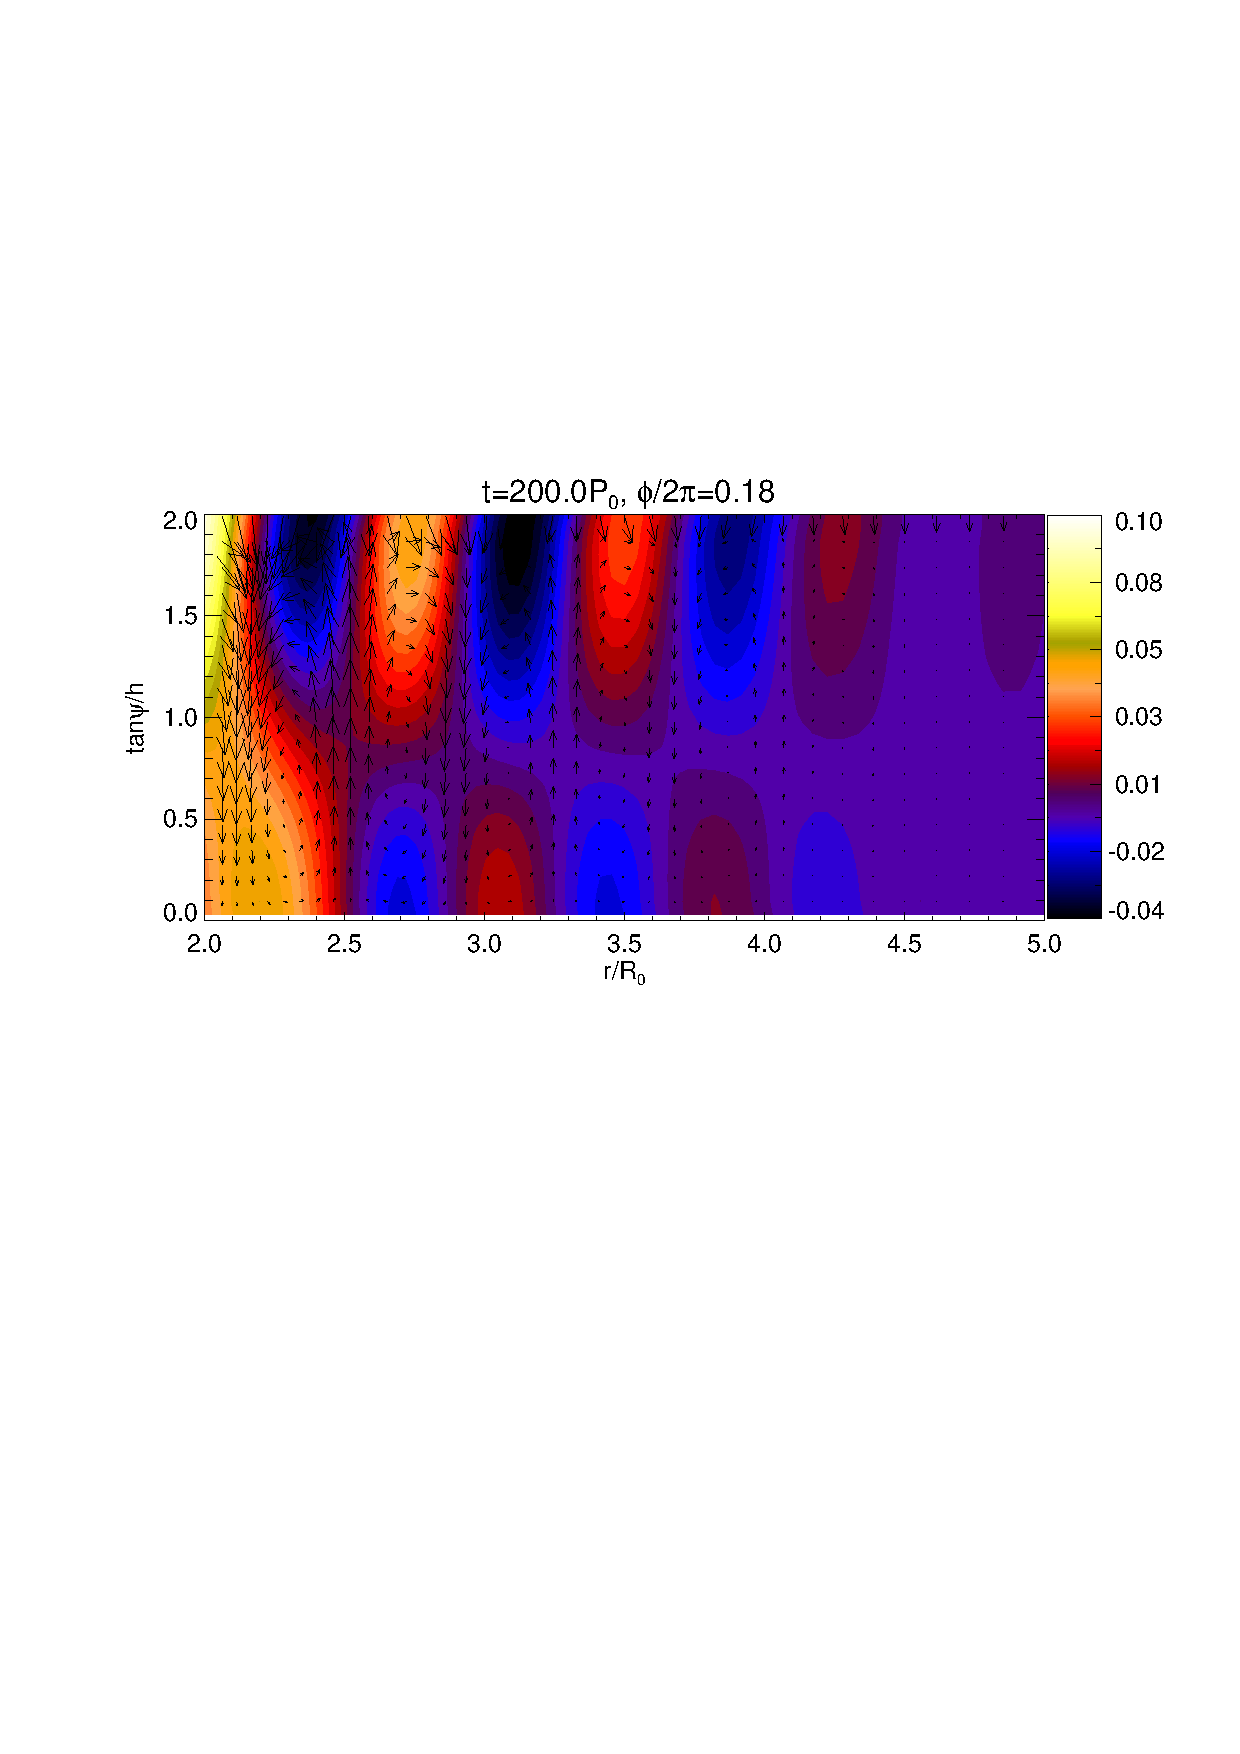
\includegraphics[scale=0.47,clip=true,trim=0cm 0cm 0cm
  0.64cm]{figures/pdisk_rz_023_nsg}  
  \caption{The $m=1$ density component in the meridional plane in the 
    PLUTO simulation. The slices are taken at the azimuth of   
    $\mathrm{max}[\Delta\rho_1(r,\pi/2,\phi)]$. Arrows represent the vector 
    $(v_r/R_0,-v_\theta/rh\sin^2{\theta})$. The top (bottom) panel corresponds
    to the inner (outer) portions of the disc. 
    \label{3d_rz}} 
\end{figure}   

Although Fig. \ref{3d_rz} appears to display significant vertical motion,
we measure the three-dimensionality parameter $\Theta < 10^{-2}$
(Eq. \ref{theta}), so vertical motions are insignificant compared to
horizontal motions. This supports a 2D approximation. On the other
hand, we find  $\mathrm{max}|v_z/c_s|\sim 0.2$ which, although
sub-sonic, is not very small.  
%may increase with height 

\subsection{Angular momentum conservation}   
Fig. \ref{3d_angmom} shows the angular momentum evolution in the 3D 
runs during the linear growth of the one-armed spiral. Because the
ZEUS-MP simulation is off-set from PLUTO, the time interval for the
plot was chosen such that the change in the angular momentum
components are comparable in the two codes. 

ZEUS-MP does not conserve angular momentum very well, but the
variation in total angular momentum $|\Delta J/J|< O(10^{-6})$ is
small compared to the individual components $|\Delta J_{0,1}/J|\sim
10^{-4}$. %it worsens with time 
PLUTO reaches similar values of $|\Delta J_{0,1}|$, but achieves better
conservation, with $|\Delta J/J|=O(10^{-8})$. These plots are again
similar to the 2D simulations, i.e. angular momentum lost by $J_1$ is
gained by $J_0$. This confirms that the interaction between $J_1$ and
$J_0$ operates in 3D and 2D similarly.  

\begin{figure}
%scale=0.41
  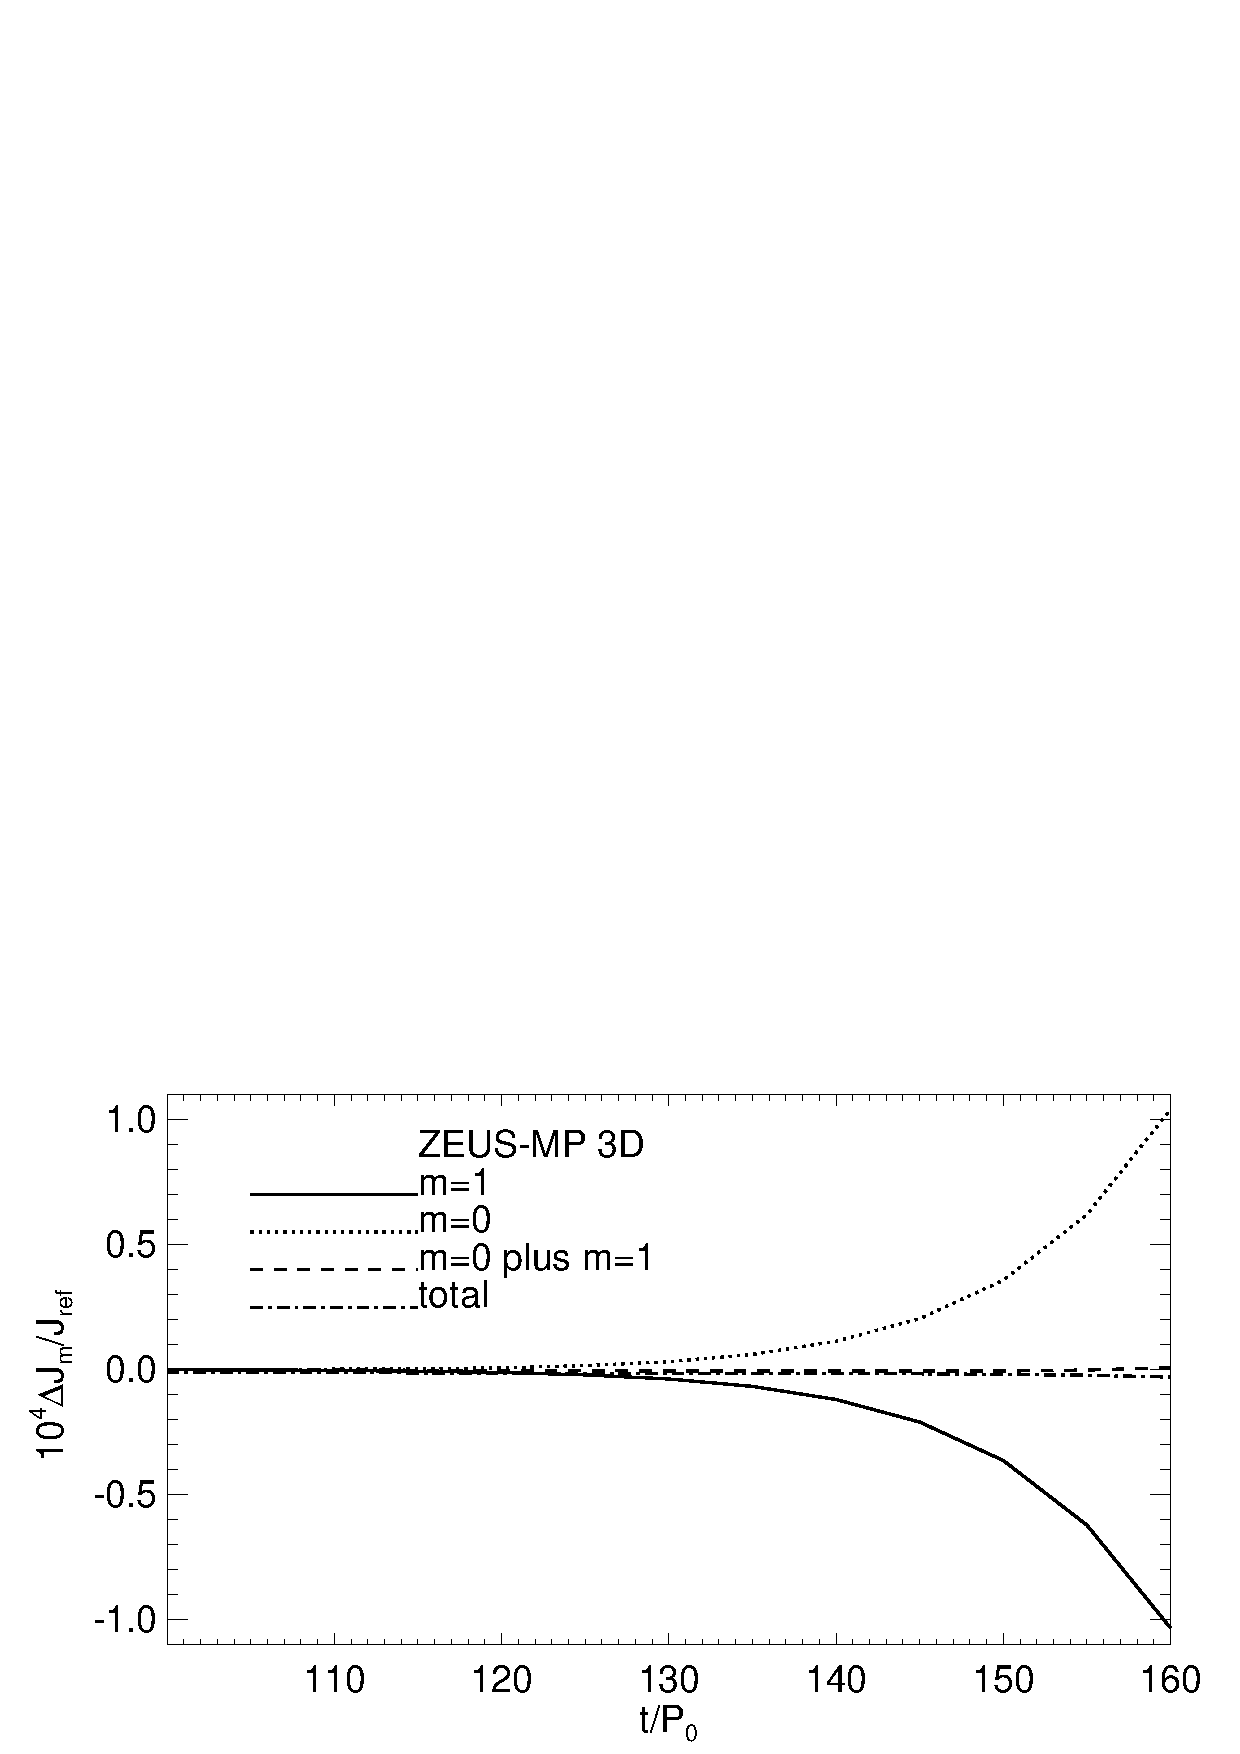
\includegraphics[scale=.41,clip=true,trim=0cm 1cm 0cm 0cm]{figures/nonaxi_evol_ang_zeus}
  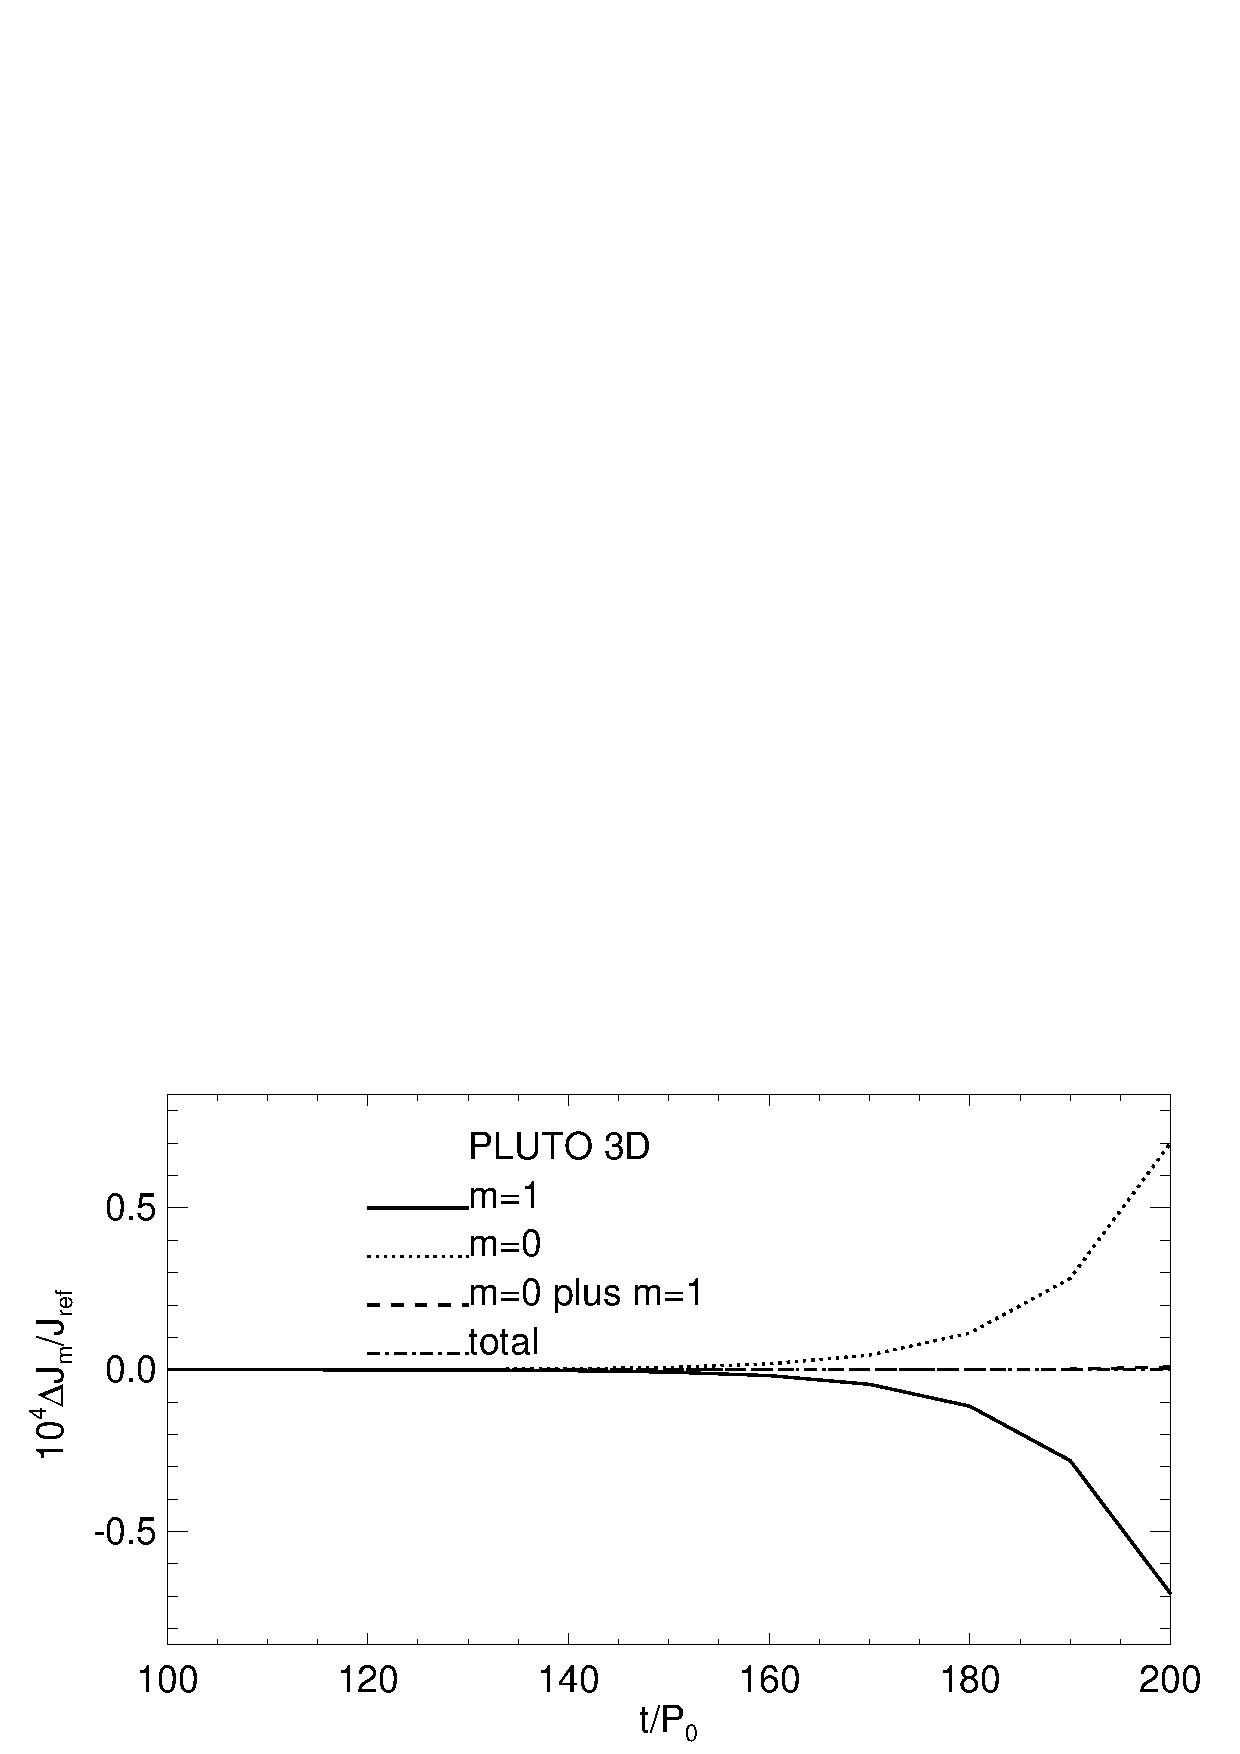
\includegraphics[scale=.41]{figures/nonaxi_evol_ang_pluto}
  \caption{Evolution of angular momentum components in the 3D 
    simulations. The perturbation 
    relative to $t=10P_0$, during the growth of the one-armed spiral,
    is shown in units of the initial total angular momentum
    $J_\mathrm{ref}$.\label{3d_angmom}}  
\end{figure}   

